\documentclass{standalone}
\usepackage{tikz}
\usetikzlibrary{patterns, positioning}
\usepackage[sfdefault]{ClearSans} %% option 'sfdefault' activates Clear Sans as the default text font
\usepackage[T1]{fontenc}

\begin{document}
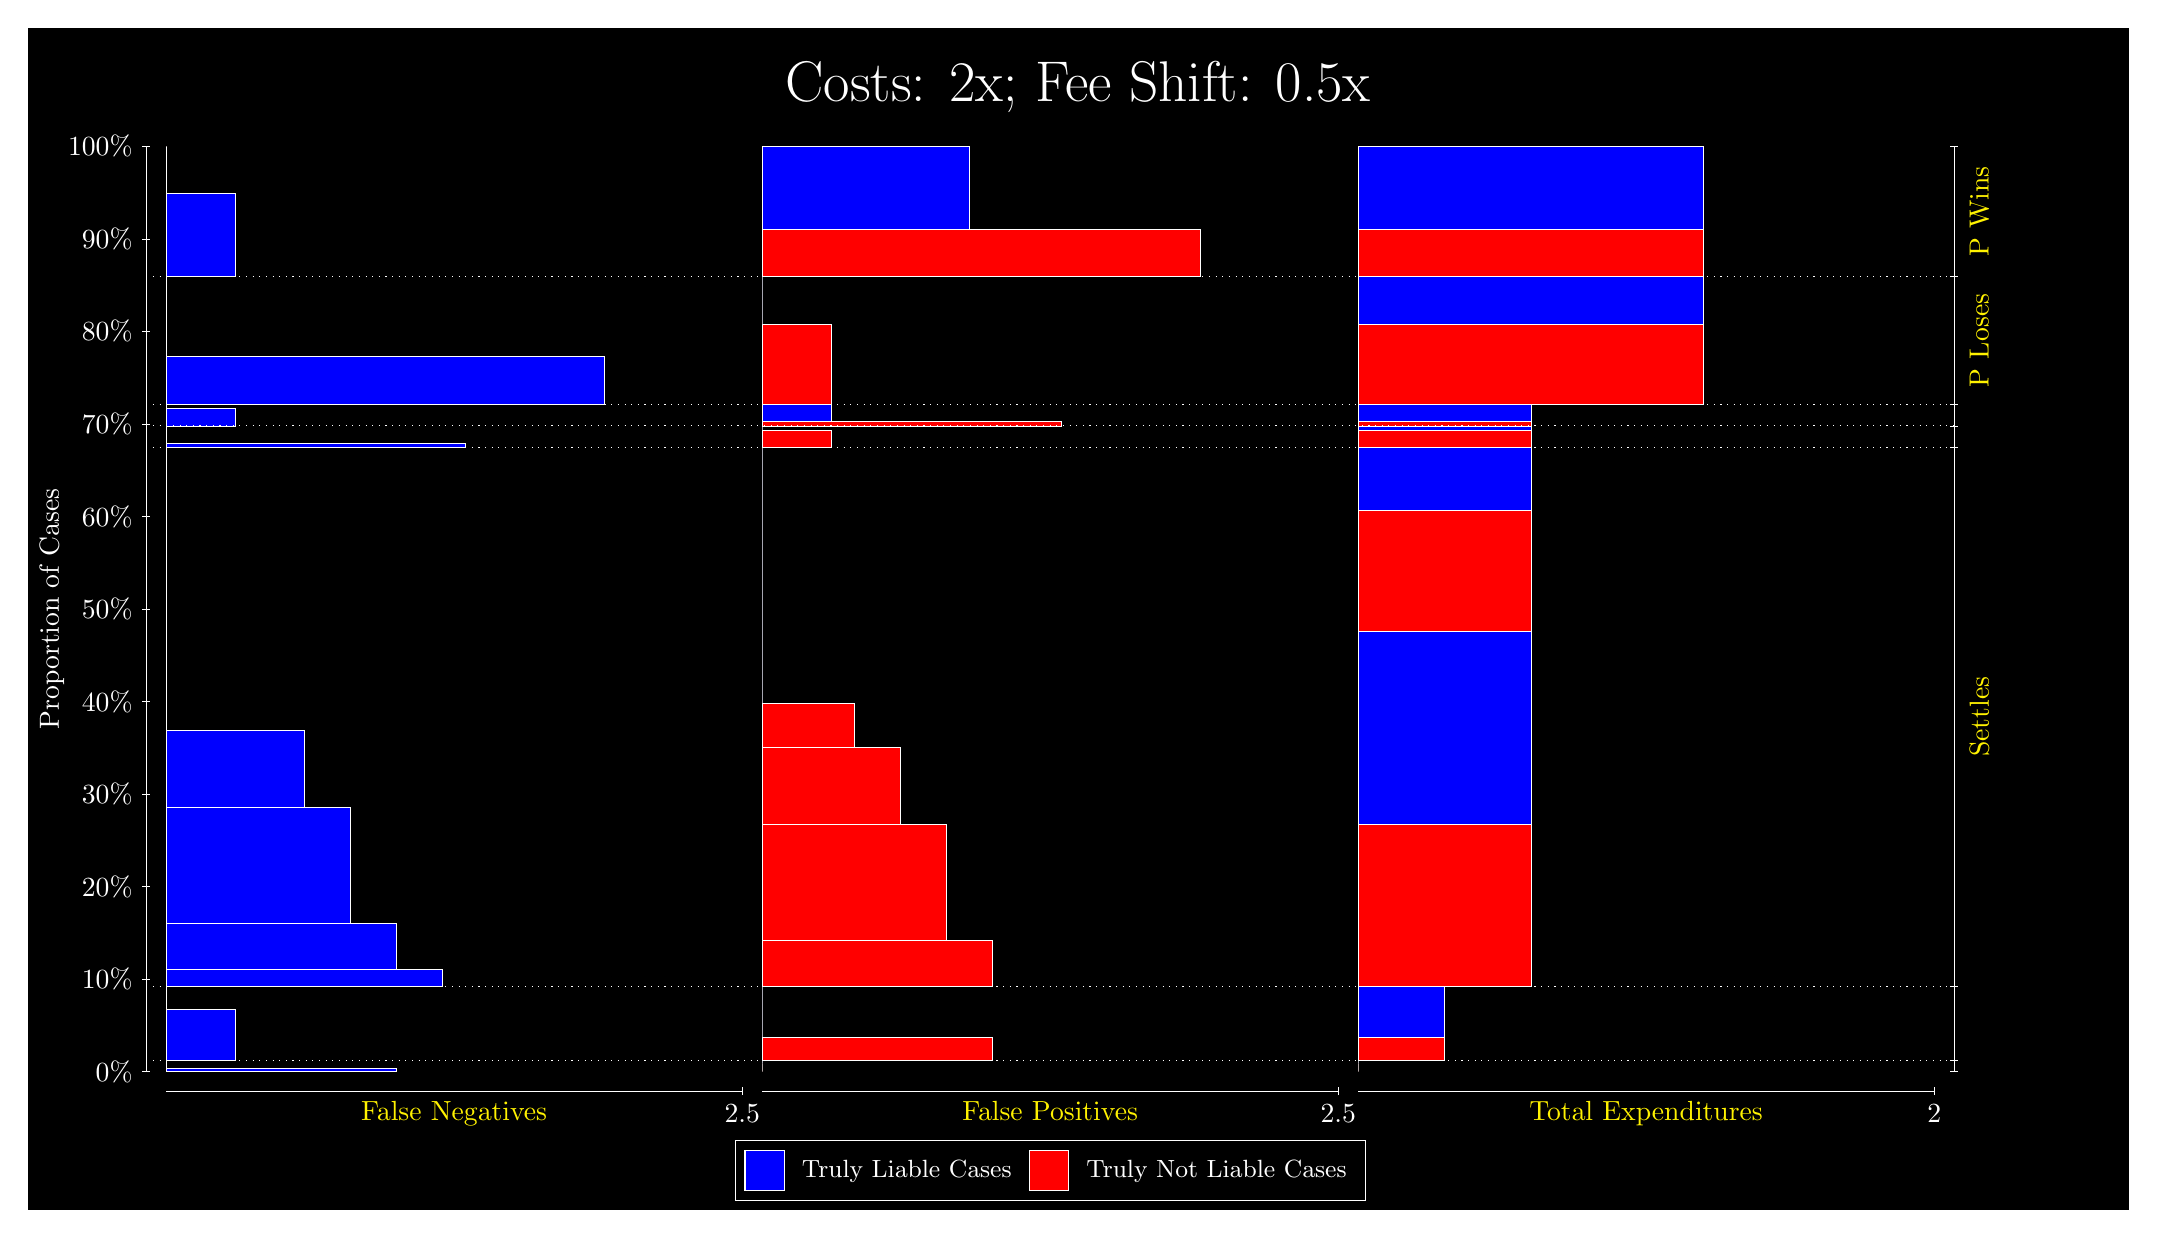
\begin{tikzpicture}
\draw[fill=black] (0,0) rectangle (26.667,15);
\draw[text=white] (0,13.5) rectangle (26.667,15) node[midway] {\huge Costs: 2x; Fee Shift: 0.5x};
\draw[white, very thin] (1.5,1.75) -- (1.5,13.5);
\node[rotate=90, text=white, anchor=center] at (0.3, 7.625) {Proportion of Cases};
\draw[white, very thin] (1.45,1.75) -- (1.55,1.75);
\node[text=white, anchor=east] at (1.45, 1.75) {0\%};
\draw[white, very thin] (1.45,2.925) -- (1.55,2.925);
\node[text=white, anchor=east] at (1.45, 2.925) {10\%};
\draw[white, very thin] (1.45,4.1) -- (1.55,4.1);
\node[text=white, anchor=east] at (1.45, 4.1) {20\%};
\draw[white, very thin] (1.45,5.275) -- (1.55,5.275);
\node[text=white, anchor=east] at (1.45, 5.275) {30\%};
\draw[white, very thin] (1.45,6.45) -- (1.55,6.45);
\node[text=white, anchor=east] at (1.45, 6.45) {40\%};
\draw[white, very thin] (1.45,7.625) -- (1.55,7.625);
\node[text=white, anchor=east] at (1.45, 7.625) {50\%};
\draw[white, very thin] (1.45,8.8) -- (1.55,8.8);
\node[text=white, anchor=east] at (1.45, 8.8) {60\%};
\draw[white, very thin] (1.45,9.975) -- (1.55,9.975);
\node[text=white, anchor=east] at (1.45, 9.975) {70\%};
\draw[white, very thin] (1.45,11.15) -- (1.55,11.15);
\node[text=white, anchor=east] at (1.45, 11.15) {80\%};
\draw[white, very thin] (1.45,12.325) -- (1.55,12.325);
\node[text=white, anchor=east] at (1.45, 12.325) {90\%};
\draw[white, very thin] (1.45,13.5) -- (1.55,13.5);
\node[text=white, anchor=east] at (1.45, 13.5) {100\%};

\draw[white, very thin] (24.457,1.75) -- (24.457,13.5);
\draw[white, very thin] (24.407,1.75) -- (24.507,1.75);
\node[anchor=west] at (24.407, 1.75) {};
\draw[white, very thin] (24.407,1.8925) -- (24.507,1.8925);
\node[anchor=west] at (24.407, 1.8925) {};
\draw[white, very thin] (24.407,2.8331) -- (24.507,2.8331);
\node[anchor=west] at (24.407, 2.8331) {};
\draw[white, very thin] (24.407,9.6766) -- (24.507,9.6766);
\node[anchor=west] at (24.407, 9.6766) {};
\draw[white, very thin] (24.407,9.9495) -- (24.507,9.9495);
\node[anchor=west] at (24.407, 9.9495) {};
\draw[white, very thin] (24.407,10.222) -- (24.507,10.222);
\node[anchor=west] at (24.407, 10.222) {};
\draw[white, very thin] (24.407,11.847) -- (24.507,11.847);
\node[anchor=west] at (24.407, 11.847) {};
\draw[white, very thin] (24.407,13.5) -- (24.507,13.5);
\node[anchor=west] at (24.407, 13.5) {};

\draw[white, very thin, fill=blue] (1.75,1.75) rectangle (4.6775,1.7891);
\draw[white, very thin, fill=red] (1.75,1.7891) rectangle (1.75,1.8925);
\draw[white, very thin, fill=blue] (1.75,1.8925) rectangle (2.6283,2.5387);
\draw[white, very thin, fill=red] (1.75,2.5387) rectangle (1.75,2.8331);
\draw[white, very thin, fill=blue] (1.75,2.8331) rectangle (5.2631,3.0481);
\draw[white, very thin, fill=blue] (1.75,3.0481) rectangle (4.6775,3.637);
\draw[white, very thin, fill=blue] (1.75,3.637) rectangle (4.092,5.1058);
\draw[white, very thin, fill=blue] (1.75,5.1058) rectangle (3.5065,6.0822);
\draw[white, very thin, fill=red] (1.75,6.0822) rectangle (1.75,9.6766);
\draw[white, very thin, fill=blue] (1.75,9.6766) rectangle (5.5558,9.7301);
\draw[white, very thin, fill=red] (1.75,9.7301) rectangle (1.75,9.9495);
\draw[white, very thin, fill=blue] (1.75,9.9495) rectangle (2.6283,10.169);
\draw[white, very thin, fill=red] (1.75,10.169) rectangle (1.75,10.222);
\draw[white, very thin, fill=blue] (1.75,10.222) rectangle (7.3123,10.832);
\draw[white, very thin, fill=red] (1.75,10.832) rectangle (1.75,11.847);
\draw[white, very thin, fill=blue] (1.75,11.847) rectangle (2.6283,12.904);
\draw[white, very thin, fill=red] (1.75,12.904) rectangle (1.75,13.5);
\draw[white, very thin, fill=red] (9.3189,1.75) rectangle (9.3189,1.8534);
\draw[white, very thin, fill=blue] (9.3189,1.8534) rectangle (9.3189,1.8925);
\draw[white, very thin, fill=red] (9.3189,1.8925) rectangle (12.246,2.1869);
\draw[white, very thin, fill=blue] (9.3189,2.1869) rectangle (9.3189,2.8331);
\draw[white, very thin, fill=red] (9.3189,2.8331) rectangle (12.246,3.422);
\draw[white, very thin, fill=red] (9.3189,3.422) rectangle (11.661,4.8908);
\draw[white, very thin, fill=red] (9.3189,4.8908) rectangle (11.075,5.8672);
\draw[white, very thin, fill=red] (9.3189,5.8672) rectangle (10.49,6.4275);
\draw[white, very thin, fill=blue] (9.3189,6.4275) rectangle (9.3189,9.6766);
\draw[white, very thin, fill=red] (9.3189,9.6766) rectangle (10.197,9.8961);
\draw[white, very thin, fill=blue] (9.3189,9.8961) rectangle (9.3189,9.9495);
\draw[white, very thin, fill=red] (9.3189,9.9495) rectangle (13.125,10.003);
\draw[white, very thin, fill=blue] (9.3189,10.003) rectangle (10.197,10.222);
\draw[white, very thin, fill=red] (9.3189,10.222) rectangle (10.197,11.237);
\draw[white, very thin, fill=blue] (9.3189,11.237) rectangle (9.3189,11.847);
\draw[white, very thin, fill=red] (9.3189,11.847) rectangle (14.881,12.442);
\draw[white, very thin, fill=blue] (9.3189,12.442) rectangle (11.954,13.5);
\draw[white, very thin, fill=red] (16.888,1.75) rectangle (16.888,1.8534);
\draw[white, very thin, fill=blue] (16.888,1.8534) rectangle (16.888,1.8925);
\draw[white, very thin, fill=red] (16.888,1.8925) rectangle (17.986,2.1869);
\draw[white, very thin, fill=blue] (16.888,2.1869) rectangle (17.986,2.8331);
\draw[white, very thin, fill=red] (16.888,2.8331) rectangle (19.083,4.8908);
\draw[white, very thin, fill=blue] (16.888,4.8908) rectangle (19.083,7.336);
\draw[white, very thin, fill=red] (16.888,7.336) rectangle (19.083,8.8727);
\draw[white, very thin, fill=blue] (16.888,8.8727) rectangle (19.083,9.6766);
\draw[white, very thin, fill=red] (16.888,9.6766) rectangle (19.083,9.8961);
\draw[white, very thin, fill=blue] (16.888,9.8961) rectangle (19.083,9.9495);
\draw[white, very thin, fill=red] (16.888,9.9495) rectangle (19.083,10.003);
\draw[white, very thin, fill=blue] (16.888,10.003) rectangle (19.083,10.222);
\draw[white, very thin, fill=red] (16.888,10.222) rectangle (21.279,11.237);
\draw[white, very thin, fill=blue] (16.888,11.237) rectangle (21.279,11.847);
\draw[white, very thin, fill=red] (16.888,11.847) rectangle (21.279,12.442);
\draw[white, very thin, fill=blue] (16.888,12.442) rectangle (21.279,13.5);
\draw[white, dotted] (1.5,1.8925) -- (24.457,1.8925);
\draw[white, dotted] (1.5,2.8331) -- (24.457,2.8331);
\draw[white, dotted] (1.5,9.6766) -- (24.457,9.6766);
\draw[white, dotted] (1.5,9.9495) -- (24.457,9.9495);
\draw[white, dotted] (1.5,10.222) -- (24.457,10.222);
\draw[white, dotted] (1.5,11.847) -- (24.457,11.847);
\draw[white, very thin] (1.75,1.5) -- (9.0689,1.5);
\node[text=yellow, anchor=north] at (5.4094, 1.5) {False Negatives};
\draw[white, very thin] (9.0689,1.45) -- (9.0689,1.55);
\node[text=white, anchor=north] at (9.0689, 1.45) {2.5};

\draw[white, very thin] (9.3189,1.5) -- (16.638,1.5);
\node[text=yellow, anchor=north] at (12.978, 1.5) {False Positives};
\draw[white, very thin] (16.638,1.45) -- (16.638,1.55);
\node[text=white, anchor=north] at (16.638, 1.45) {2.5};

\draw[white, very thin] (16.888,1.5) -- (24.207,1.5);
\node[text=yellow, anchor=north] at (20.547, 1.5) {Total Expenditures};
\draw[white, very thin] (24.207,1.45) -- (24.207,1.55);
\node[text=white, anchor=north] at (24.207, 1.45) {2};



\node[text=yellow, centered, rotate=90] at (24.777, 6.2549) {Settles};


\node[text=yellow, centered, rotate=90] at (24.777, 11.035) {P Loses};
\node[text=yellow, centered, rotate=90] at (24.777, 12.673) {P Wins};

\draw (12.978300999999998,1.5) node[draw=none] (baseCoordinate) {};
\begin{scope}[align=center]
        \matrix[scale=0.5, draw=white, below=0.5cm of baseCoordinate, nodes={draw}, column sep=0.1cm]{
            \node[rectangle, draw, minimum width=0.5cm, minimum height=0.5cm, fill=blue] {}; &
            \node[draw=none, font=\small, text=white] (B) {Truly Liable Cases}; &
            \node[rectangle, draw, minimum width=0.5cm, minimum height=0.5cm, fill=red] {}; &
            \node[draw=none, font=\small, text=white] (B) {Truly Not Liable Cases}; \\
            };
\end{scope}

\end{tikzpicture}
\end{document}